%!TEX root = ../Thesis.tex
\chapter{System Implementation}
The following section provides an in-depth examination of the implementation process of the designed system. It outlines the technical details of the local development setup, deployment options, and the implementation of various algorithms used within the system. In addition, it explains the communication protocols employed between different services within the system and the implementation observability of the system. The system is developed using robust coding practices and industry-standard development tools. The project employs a continuous integration and continuous deployment model, in which code changes are automatically deployed to both cloud and on-premises instances following modifications to the source code, as depicted in Appendix \ref{sec:app_07}.

\section{Local development}
\begin{figure}[H]
    \centering
    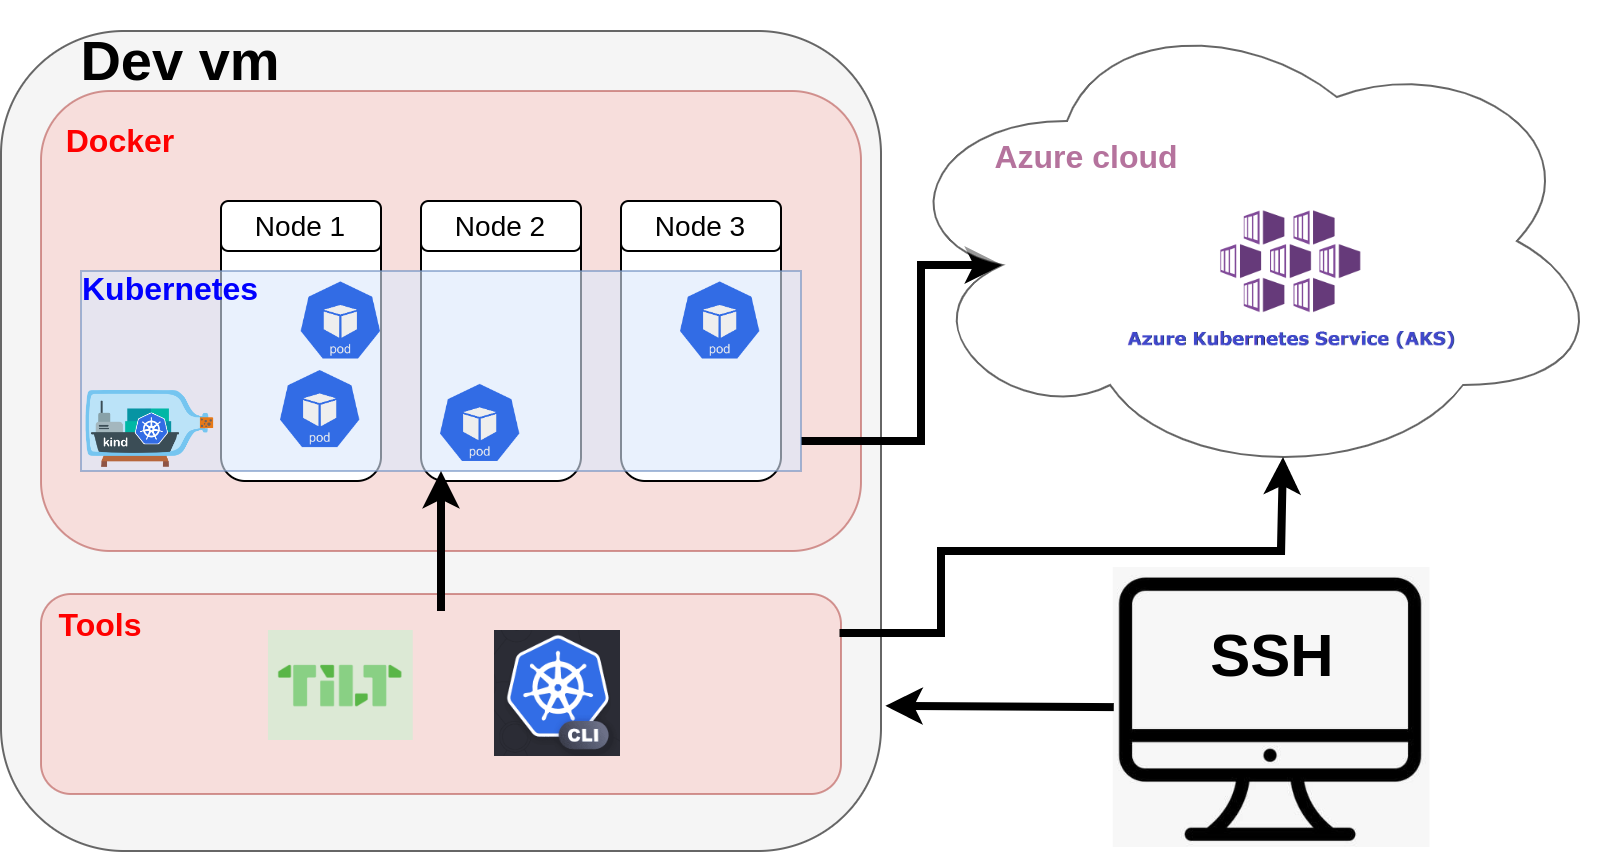
\includegraphics[width=0.8\textwidth]{pictures/development_setup.png}
    \caption{ Local development }
    \label{fig:local_development}
\end{figure}

\section{Kubernetes}
Whole project is designed to be deployed in the cloud and in particular in KaaS(kubernetes as a service) solution. For comparison of most popular cloud providers, open-sourced cost calculator\cite{managed_kubernetes_pricing} was used. Result for most popular cloud provider: amazon web services(AWS), azure(AKS), google cloud(GKE) and digital ocean(DO) can be seen on plot below:

\begin{figure}[H]
    \centering
    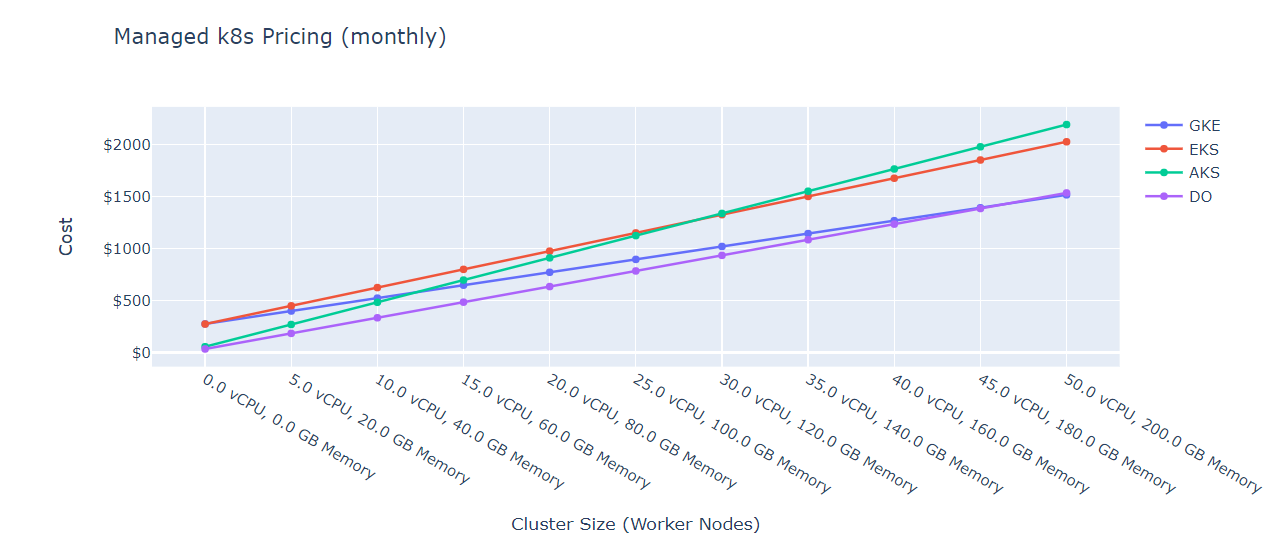
\includegraphics[width=01\textwidth]{pictures/k8s_cost.png}
    \caption{ Local development }
    \label{fig:k8s_cost}
\end{figure}

Cheapest options for small scale projects are digital ocean and azure because they doesn't charge for the compute used for the control plane. For large projects Google Cloud is the most affordable. 

Two cloud  providers were tested for this implementation: Microsoft azure and Okteto Cloud. Both are offering kubernetes as a service, but they have chosen different approaches. 

In azure kubernetes cluster is being created and then it is mostly managed by the user. It is harder to maintain but also more flexible as cluster can be scaled and extended easily.  

Okteto cloud has taken different approach, it is focused on crating development enviroment which is usually not production ready. In free tier they provide namescpace in a cluster(fully managed by okteto) with possibility to deploy up to 10 pods with limitations mentioned below:
\begin{itemize}
    \item Namespaces: 5
    \item Pods: 10
    \item CPU: 1 / pod
    \item Memory: 3Gi / pod
    \item Storage: 5Gi
\end{itemize}

Bottom line: Okteto for development azure for pruductization.

\section{Algorithms implementation}
\begin{figure}[H]
    \centering
    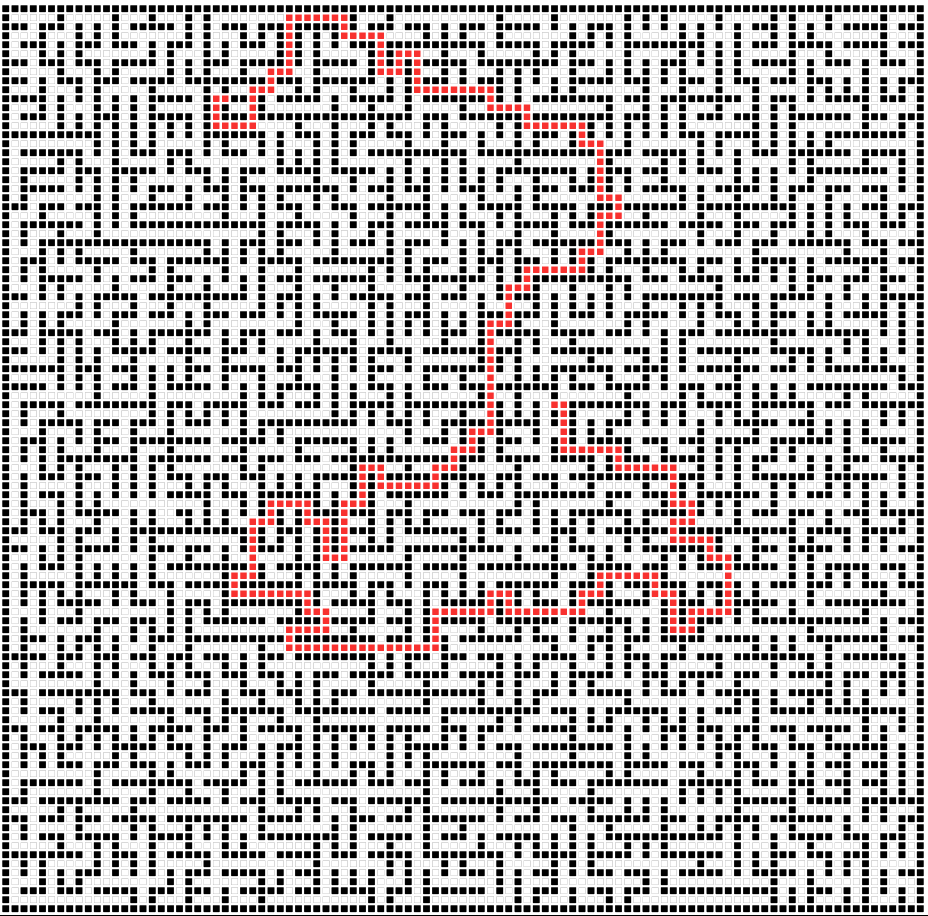
\includegraphics[width=0.8\textwidth]{pictures/single_path_maze.png}
    \caption{ Single agent path planning example} 
    \label{fig:single_agent_path}
\end{figure}

\section{Broker}
To allow the broker to be cloud agnostic, it was deployed as a container. Two main open-source projects were considered Eclipse Mosquitto and HiveMQ Community Edition, both implementing MQTT (Message Queuing Telemetry Transport) protocol.

Differences between the two include:

\begin{itemize}
    \item Mosquitto is fully open-sourced and maintained by Eclipse Foundation. HiveMQ is an enterprise product with a free community edition version.
    \item HiveMQ is better suited for a large-scale project, whereas mosquito is designed for small to medium-sized projects.
    \item HiveMQ has more features but most of them are not included in the community edition.
    \item Mosquito includes free implementation of MQTT bridge - the connection between two MQTT brokers that allows them to exchange messages with each other.
\end{itemize}

Both brokers were deployed and tested. HiveMQ was easier to manage and deploy to the Kubernetes cluster, but Mosquito was faster and more reliable. The feature which decided on choosing mosquito as a broker in this project is the implementation of the MQTT bridge which allows easy connect local and cloud brokers together and isolates traffic between cloud and local deployments.

\section{Observability}
\label{sec:04_06_observability}
Observability is the ability to check and visualize the state of the overall system. It is especially important with microservice architecture as complexity is increasing along with the decoupling of the services. There are also multiple data sources that need to be combined together to provide insight into component interactions. 

Figure \ref{fig:observability_system} shows the design of the observability system for this project. In a standard cloud-based application, all metrics are directly scraped by metric scrapers, which was implemented in a local setup. In a real system, some components are not deployed in the cloud(f.e agents) and therefore metrics need to be transported to the service which is deployed in the cloud - in this case, the backend service. Later those metrics are exposed to the metric collector.

\begin{figure}[H]
    \centering
    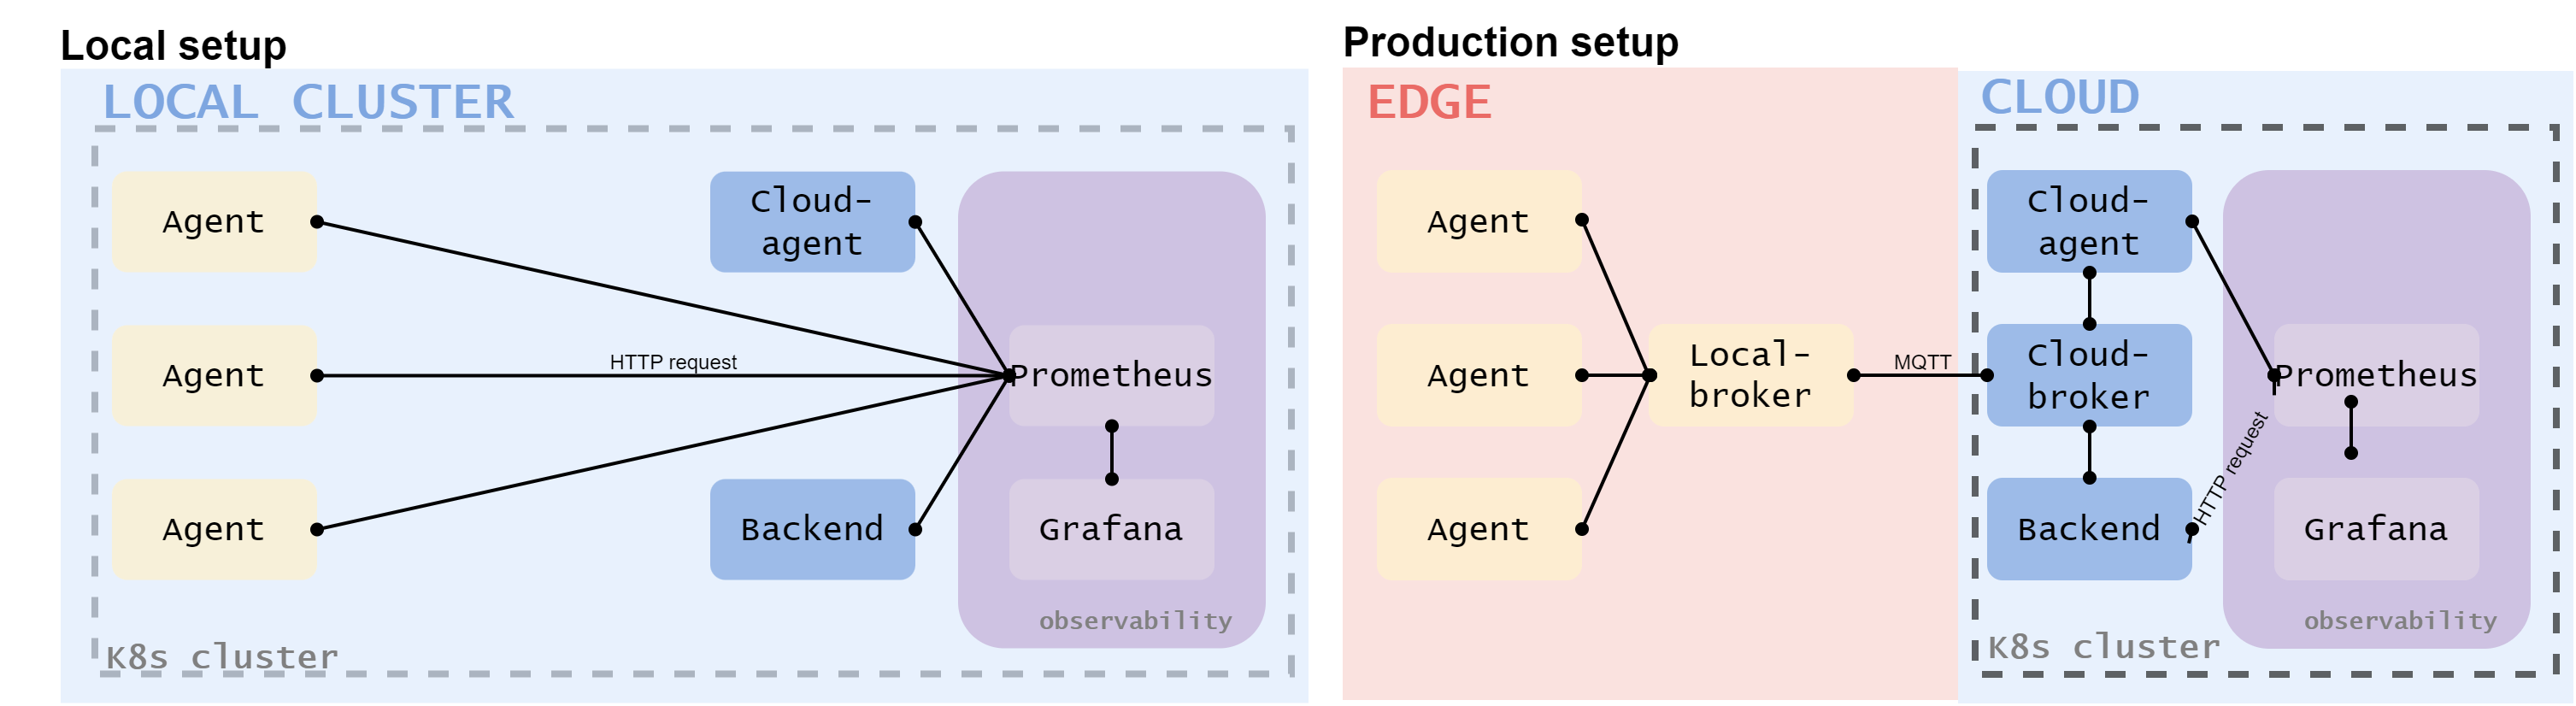
\includegraphics[width=\textwidth]{pictures/observability.png}
    \caption{ Observability design }
    \label{fig:observability_system}
\end{figure}

Two open-source components are used in order to create an observability stack: Grafana and Prometheus. Prometheus is a monitoring solution that scrapes metrics from the HTTP endpoint, in the case of Kubernetes it scrapes metrics from pods whose metric monitor service is exposed. Prometheus later stores collected data in a time-series database and provide a way to query the data using the specific language (Prometheus Query Language)\cite{prometheus_docs}.

Grafana is meant as a visualization tool. It uses Prometheus queries to show data in form of charts, graphs, and other visualizations. In this project, multiple grafana dashboards were created to monitor the status of the system and the performance of the solution. An example can be seen in figure \ref{fig:dashboard_grafana}.

\begin{figure}[H]
    \centering
    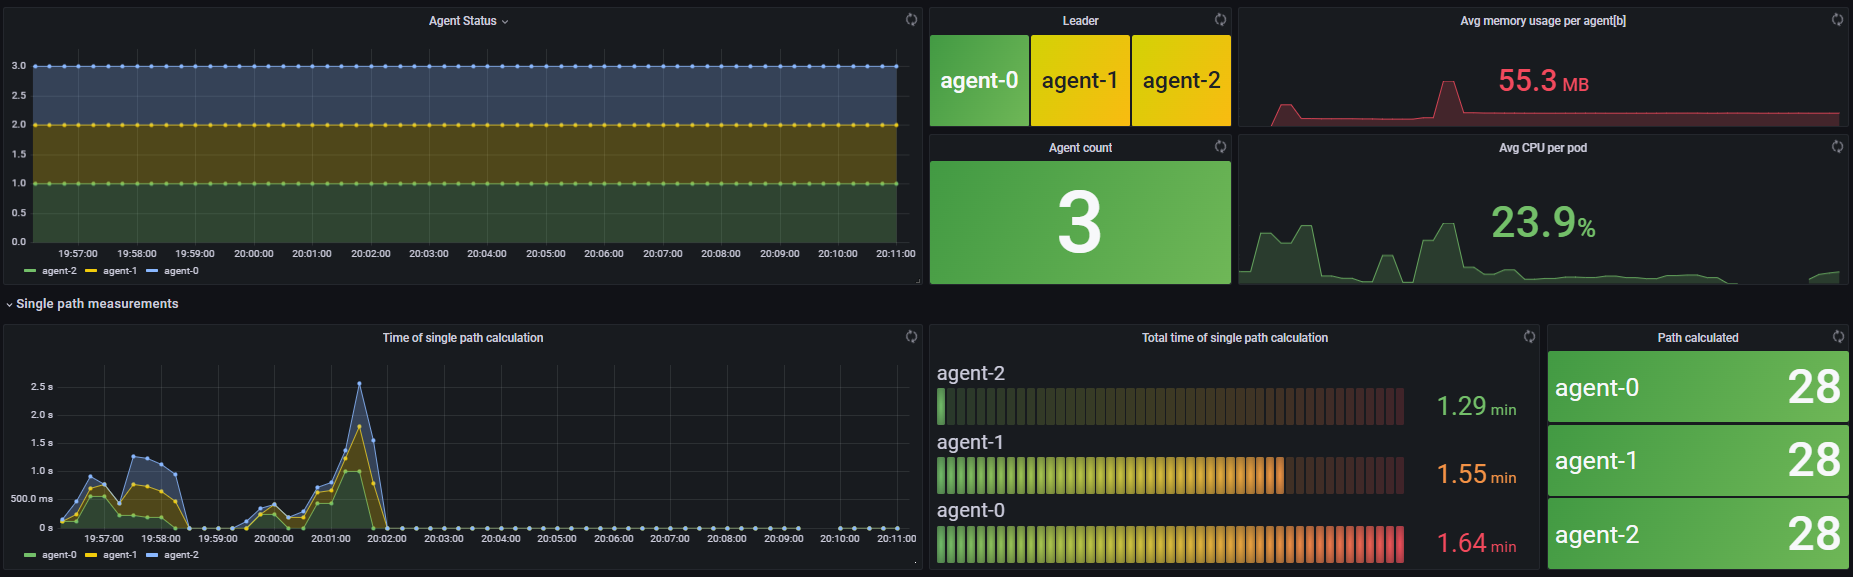
\includegraphics[width=\textwidth]{pictures/grafana.png}
    \caption{ Dashboard in grafana }
    \label{fig:dashboard_grafana}
\end{figure}

It is visualizing:
\begin{itemize}
    \item agents uptime
    \item current leader
    \item average agent memory utilization
    \item average agent CPU utilization
    \item time of path calculation
    \item number of path found
\end{itemize}



\section{Visualization}
\begin{figure}[H]
    \centering
    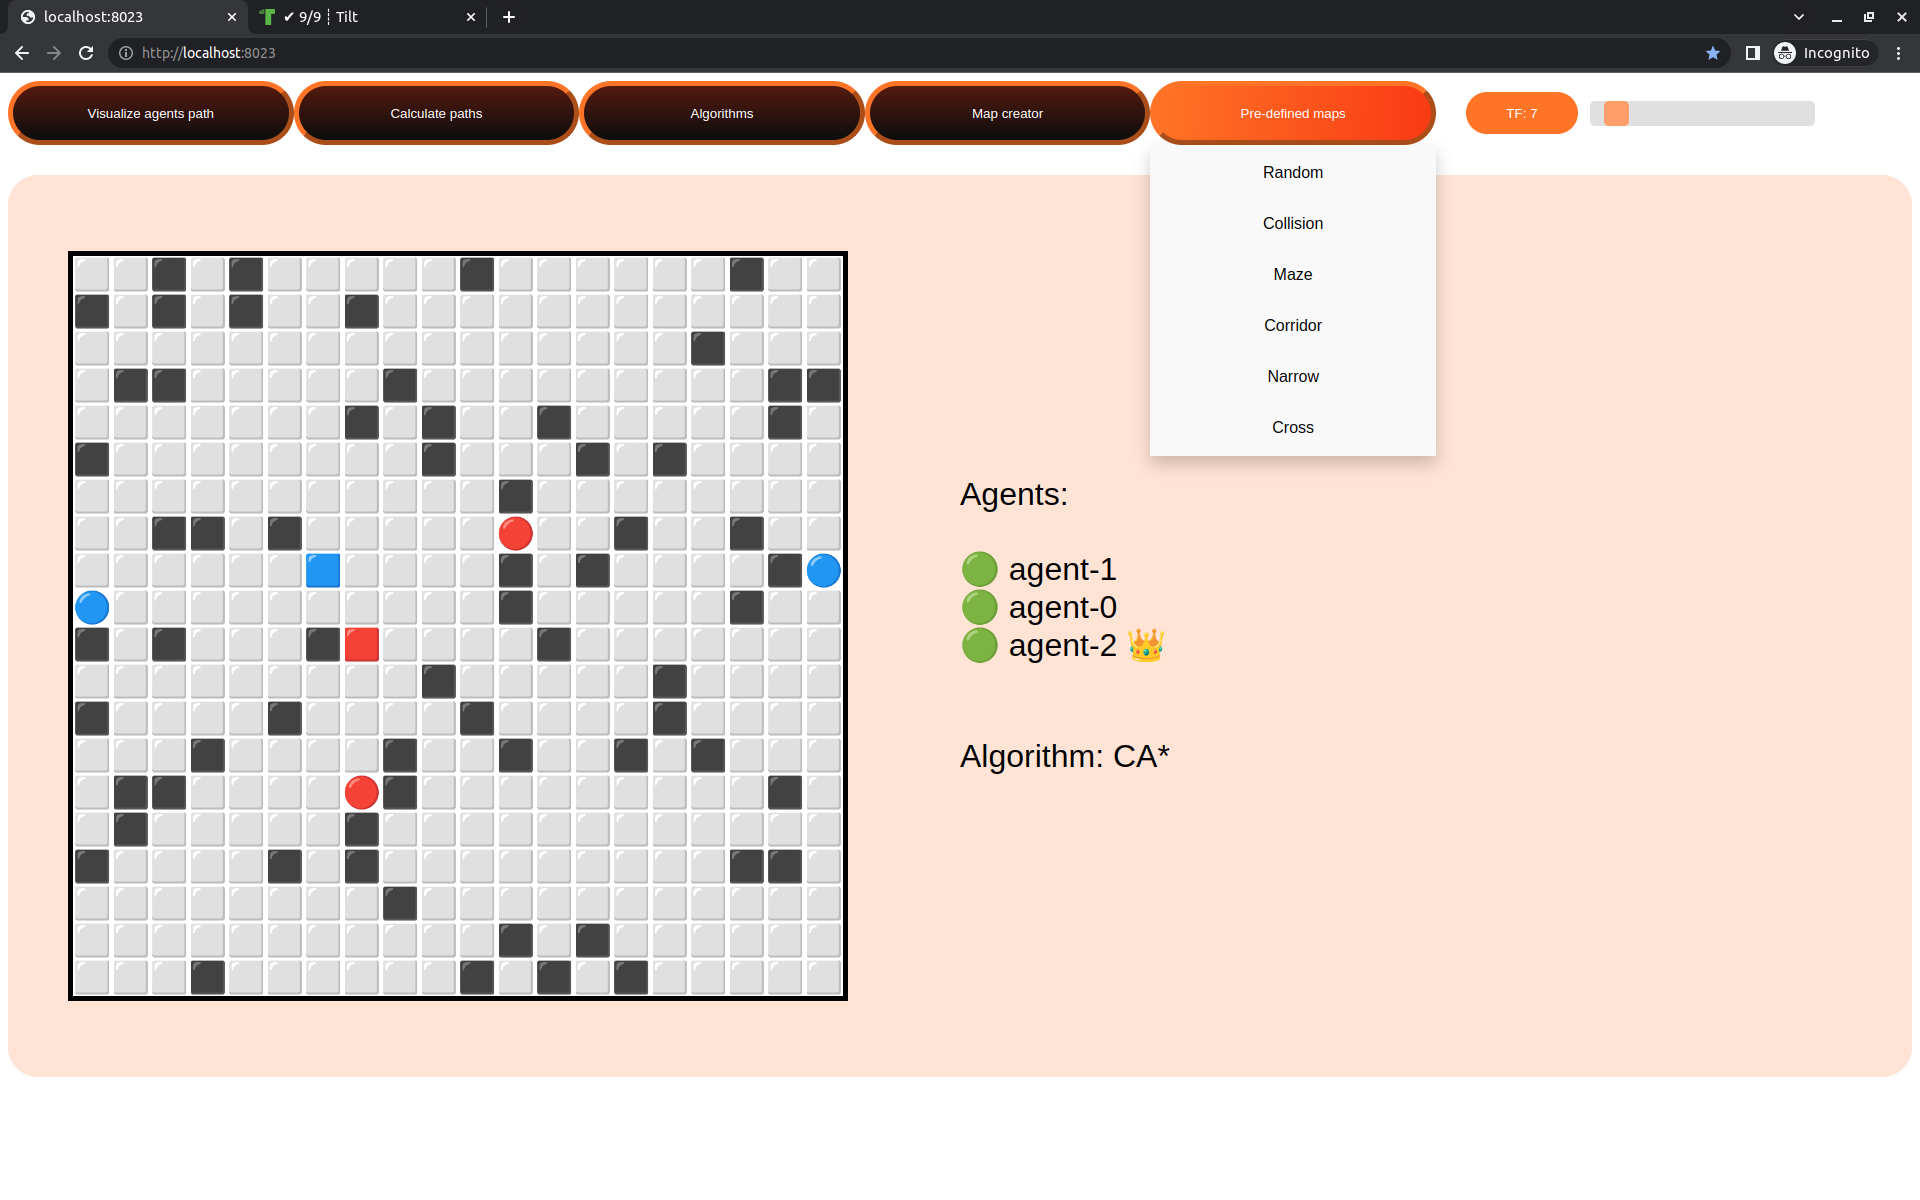
\includegraphics[width=0.8\textwidth]{pictures/frontend.png}
    \caption{ Frontend website } 
    \label{fig:frontend}
\end{figure}
